\chapter{Auswertung}
\section{Bestimmung des Kalibrierfaktors}
Da bedingt durch die Spulengeometrie das Feld innerhalb der langen Spule quantitativerseits Stärker und qualitativerseits
homogener als jenes der kurzen Spulen zu erwarten ist, dienen die Messungen an der langen Spule zur Ermittlung eines
Kalibrierfaktors $k$.\par
Mit Hilfe des Kalibrierfaktors lässt sich aus den gemessenen Ausschlägen die Feldstärke der kurzen Spulen gemäß 
\begin{equation}
    k=\frac{\Delta A}{\Delta H} \quad \Leftrightarrow \quad H=\frac{A}{k}
    \label{eq:k}
\end{equation}
ermitteln.

\begin{figure}[H]
    \centering
    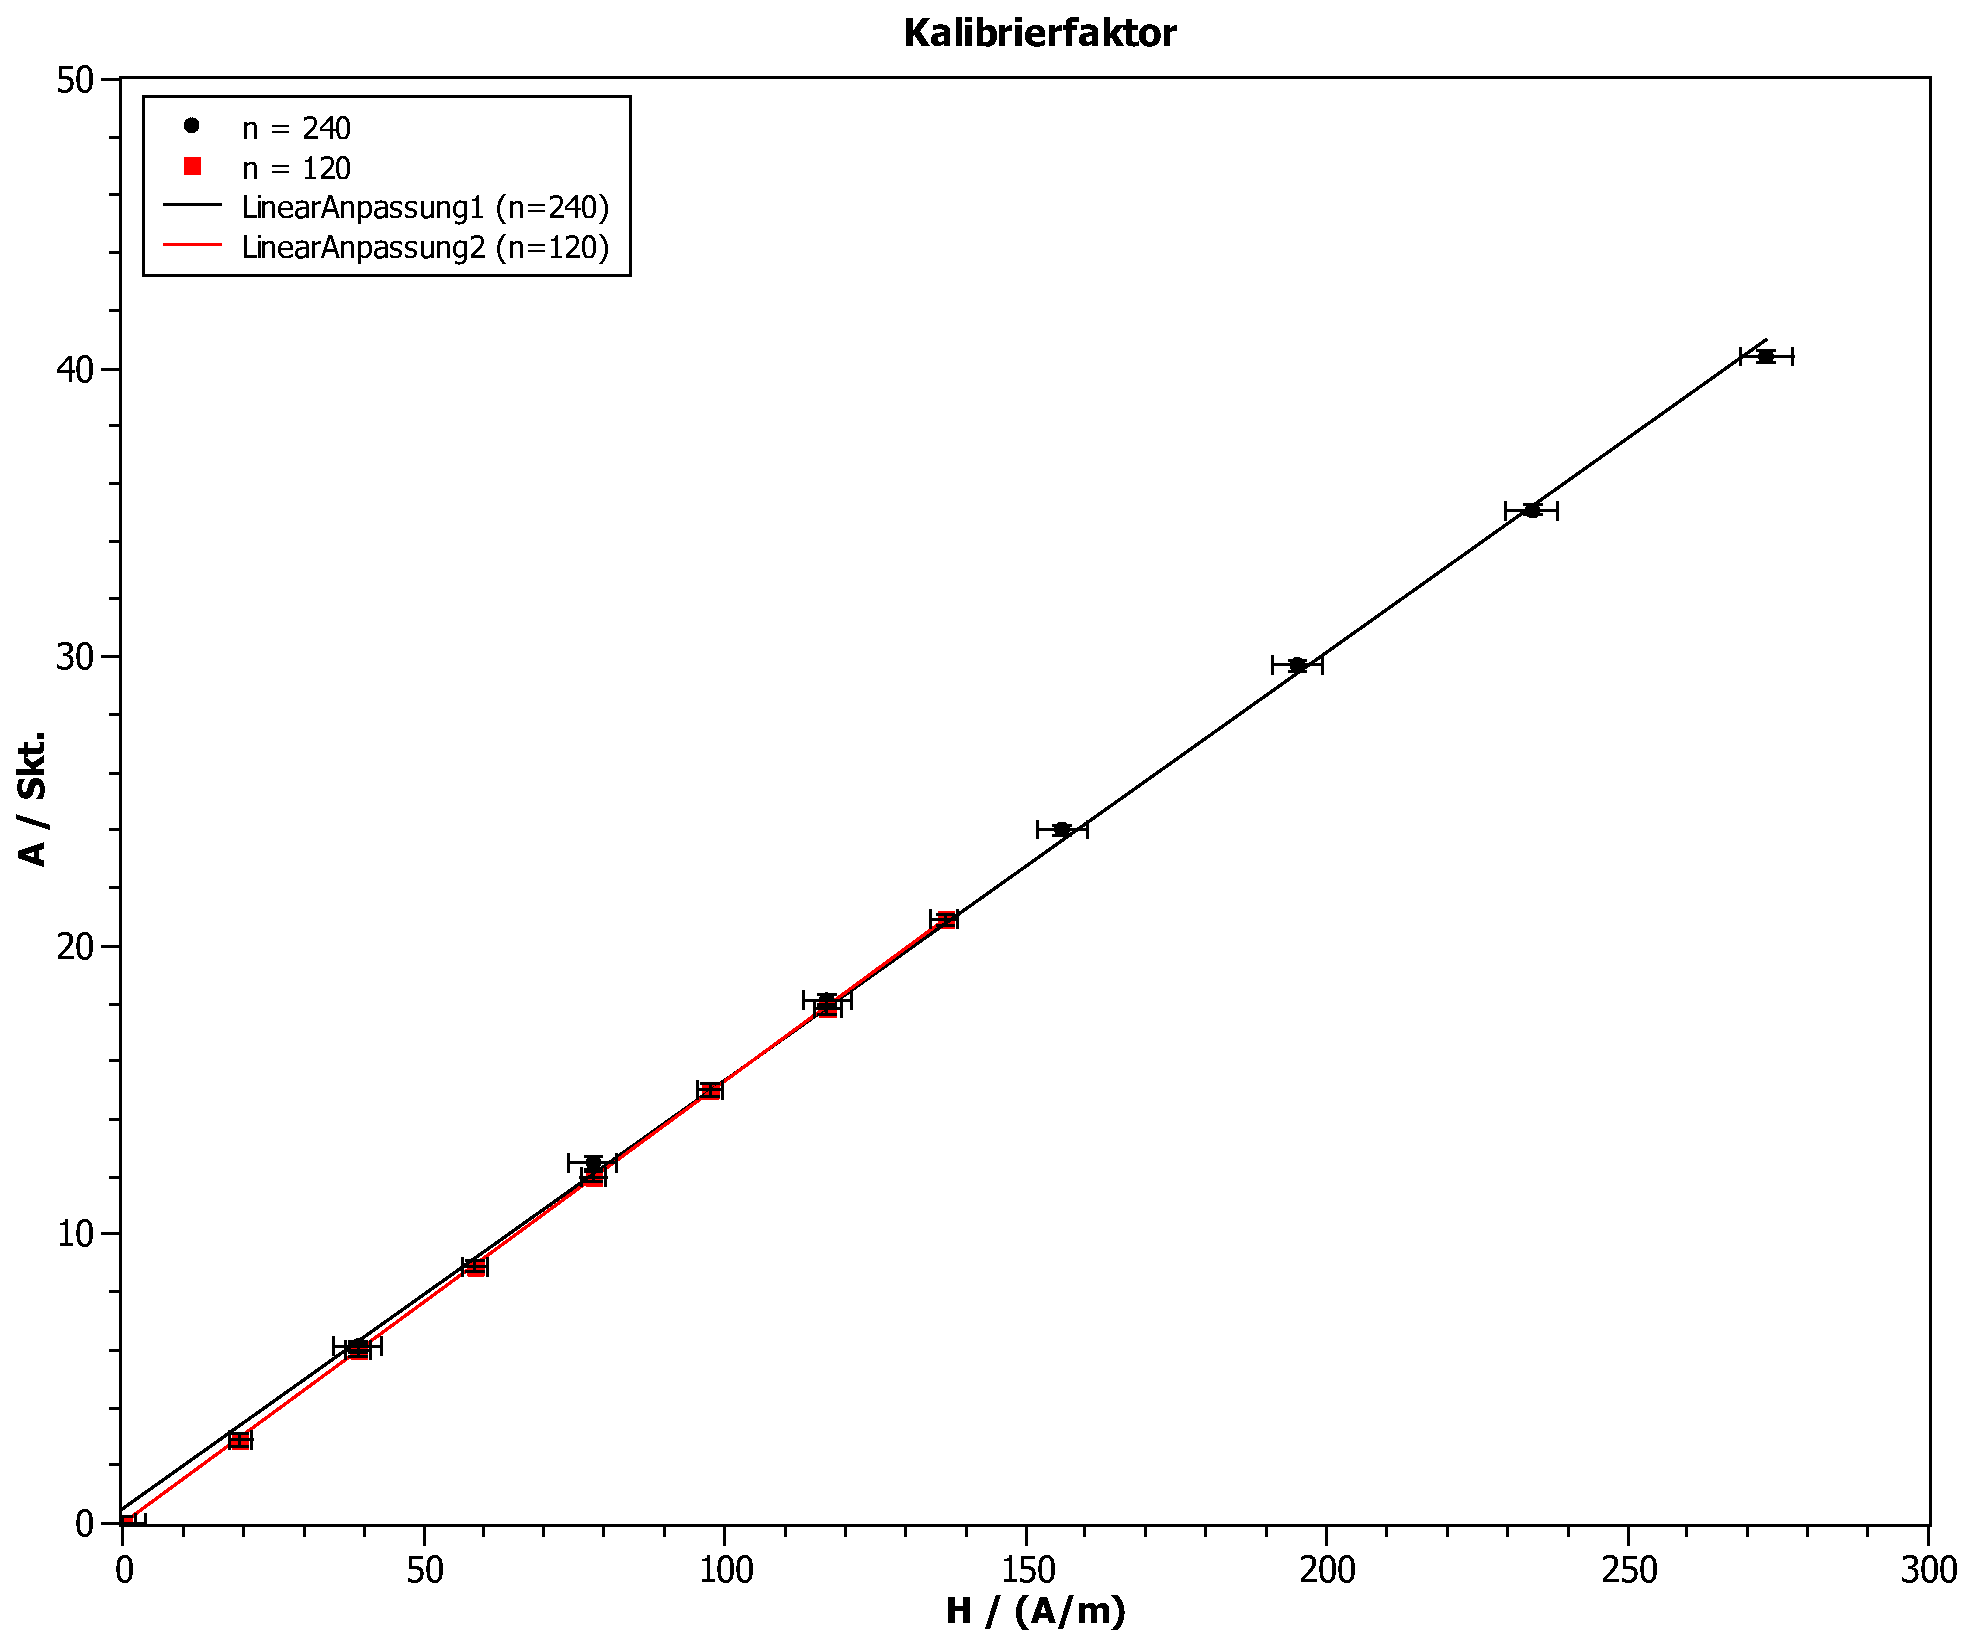
\includegraphics[width=.7\textwidth]{Kalibrierfaktor.pdf}
    \caption[Ermittlung des Kalibrierfaktors]{Ermittlung des Kalibrierfaktors als Steigung von $H_{l}(I)$ mittels \textsc{SciDavis} zur weiteren Auswertung der kurzen Spulen.}
    \label{fig:kalib}
\end{figure}

Wird der Spulenstrom $ I $ der langen Spule nach \gl{eq:3} in die magnetische Feldstärke $ H $ umgerechnet und der Skalenwert
$ A $ als Funktion von $ H $ in ein Diagramm (vgl. \bild{fig:kalib}) aufgetragen, so ergibt sich als Steigung der linearen
Anpassung der Kalibrierfaktor $ k $ mit der Abweichung $ \Delta k $

\begin{equation} 
    k = (0,151 \pm 0,002)\SI{}{\frac{Skt\cdot m}{A}}
\end{equation}

\section{Bestimmung des Proportionalitätsfaktors}

\begin{figure}[H]
    \hspace{-5mm}
    \centering
    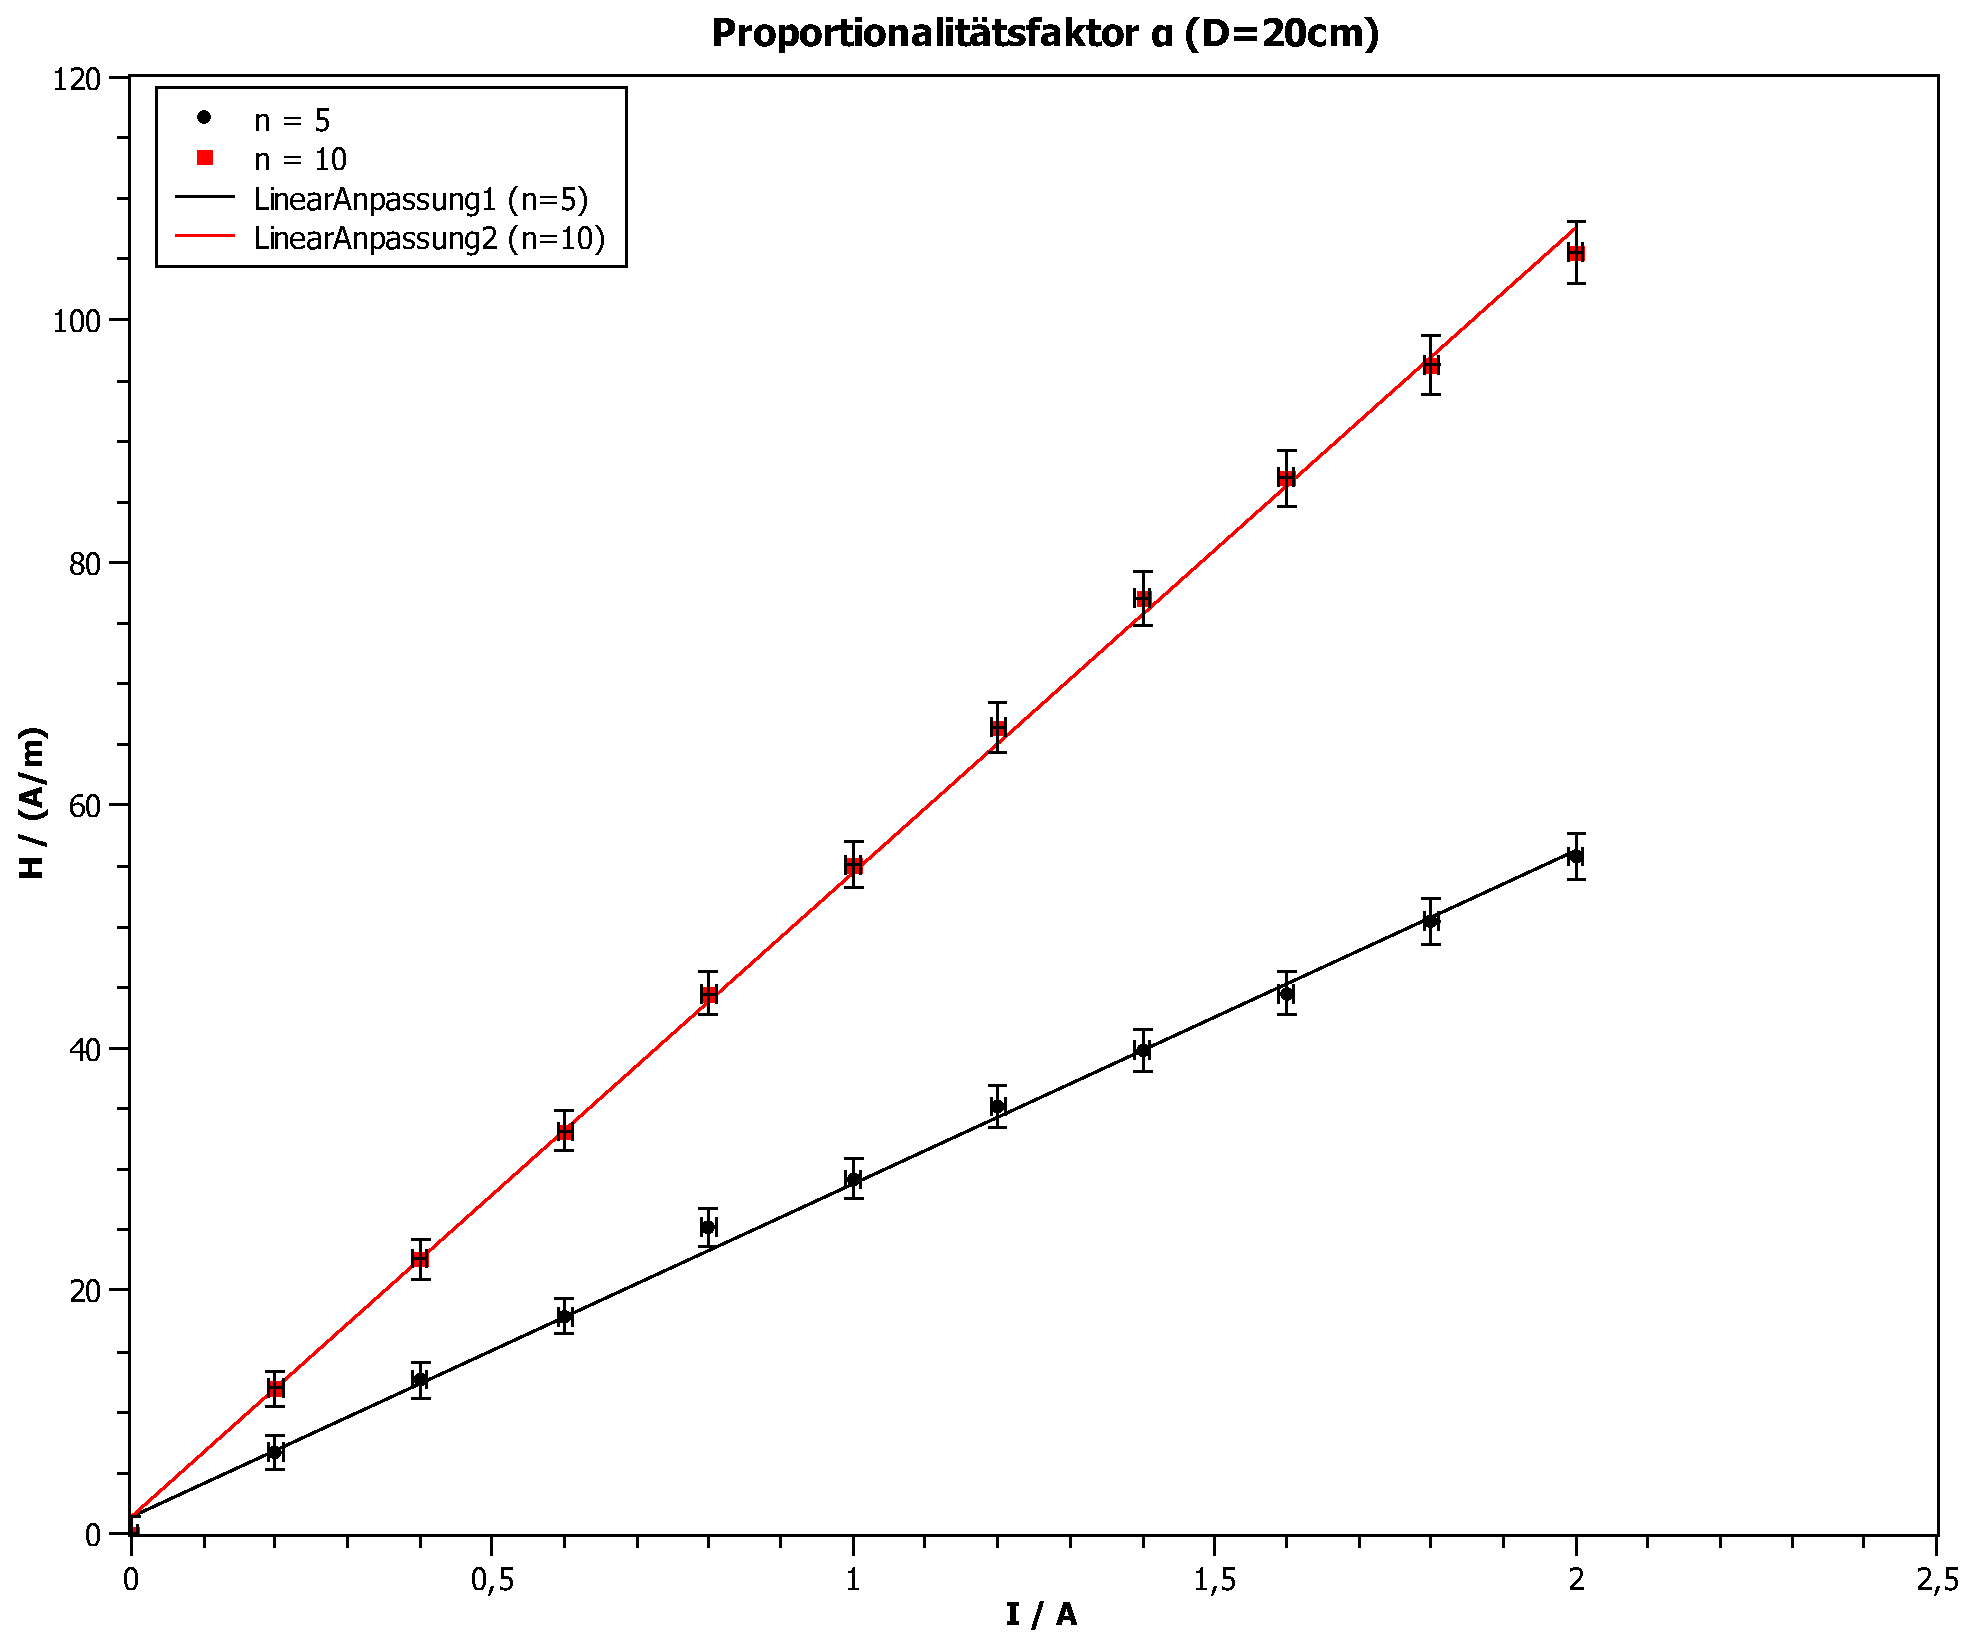
\includegraphics[width=.7\textwidth]{prop20.pdf}
    \caption[Proportionalitätsfaktor für D=20cm]{Proportionalitätsfaktor $\alpha$ für die kurze Spule mit $D=\SI{20}{cm}$.}
    \label{fig:20prop}
\end{figure}

\par\bigskip

\begin{figure}[H]
    \centering
    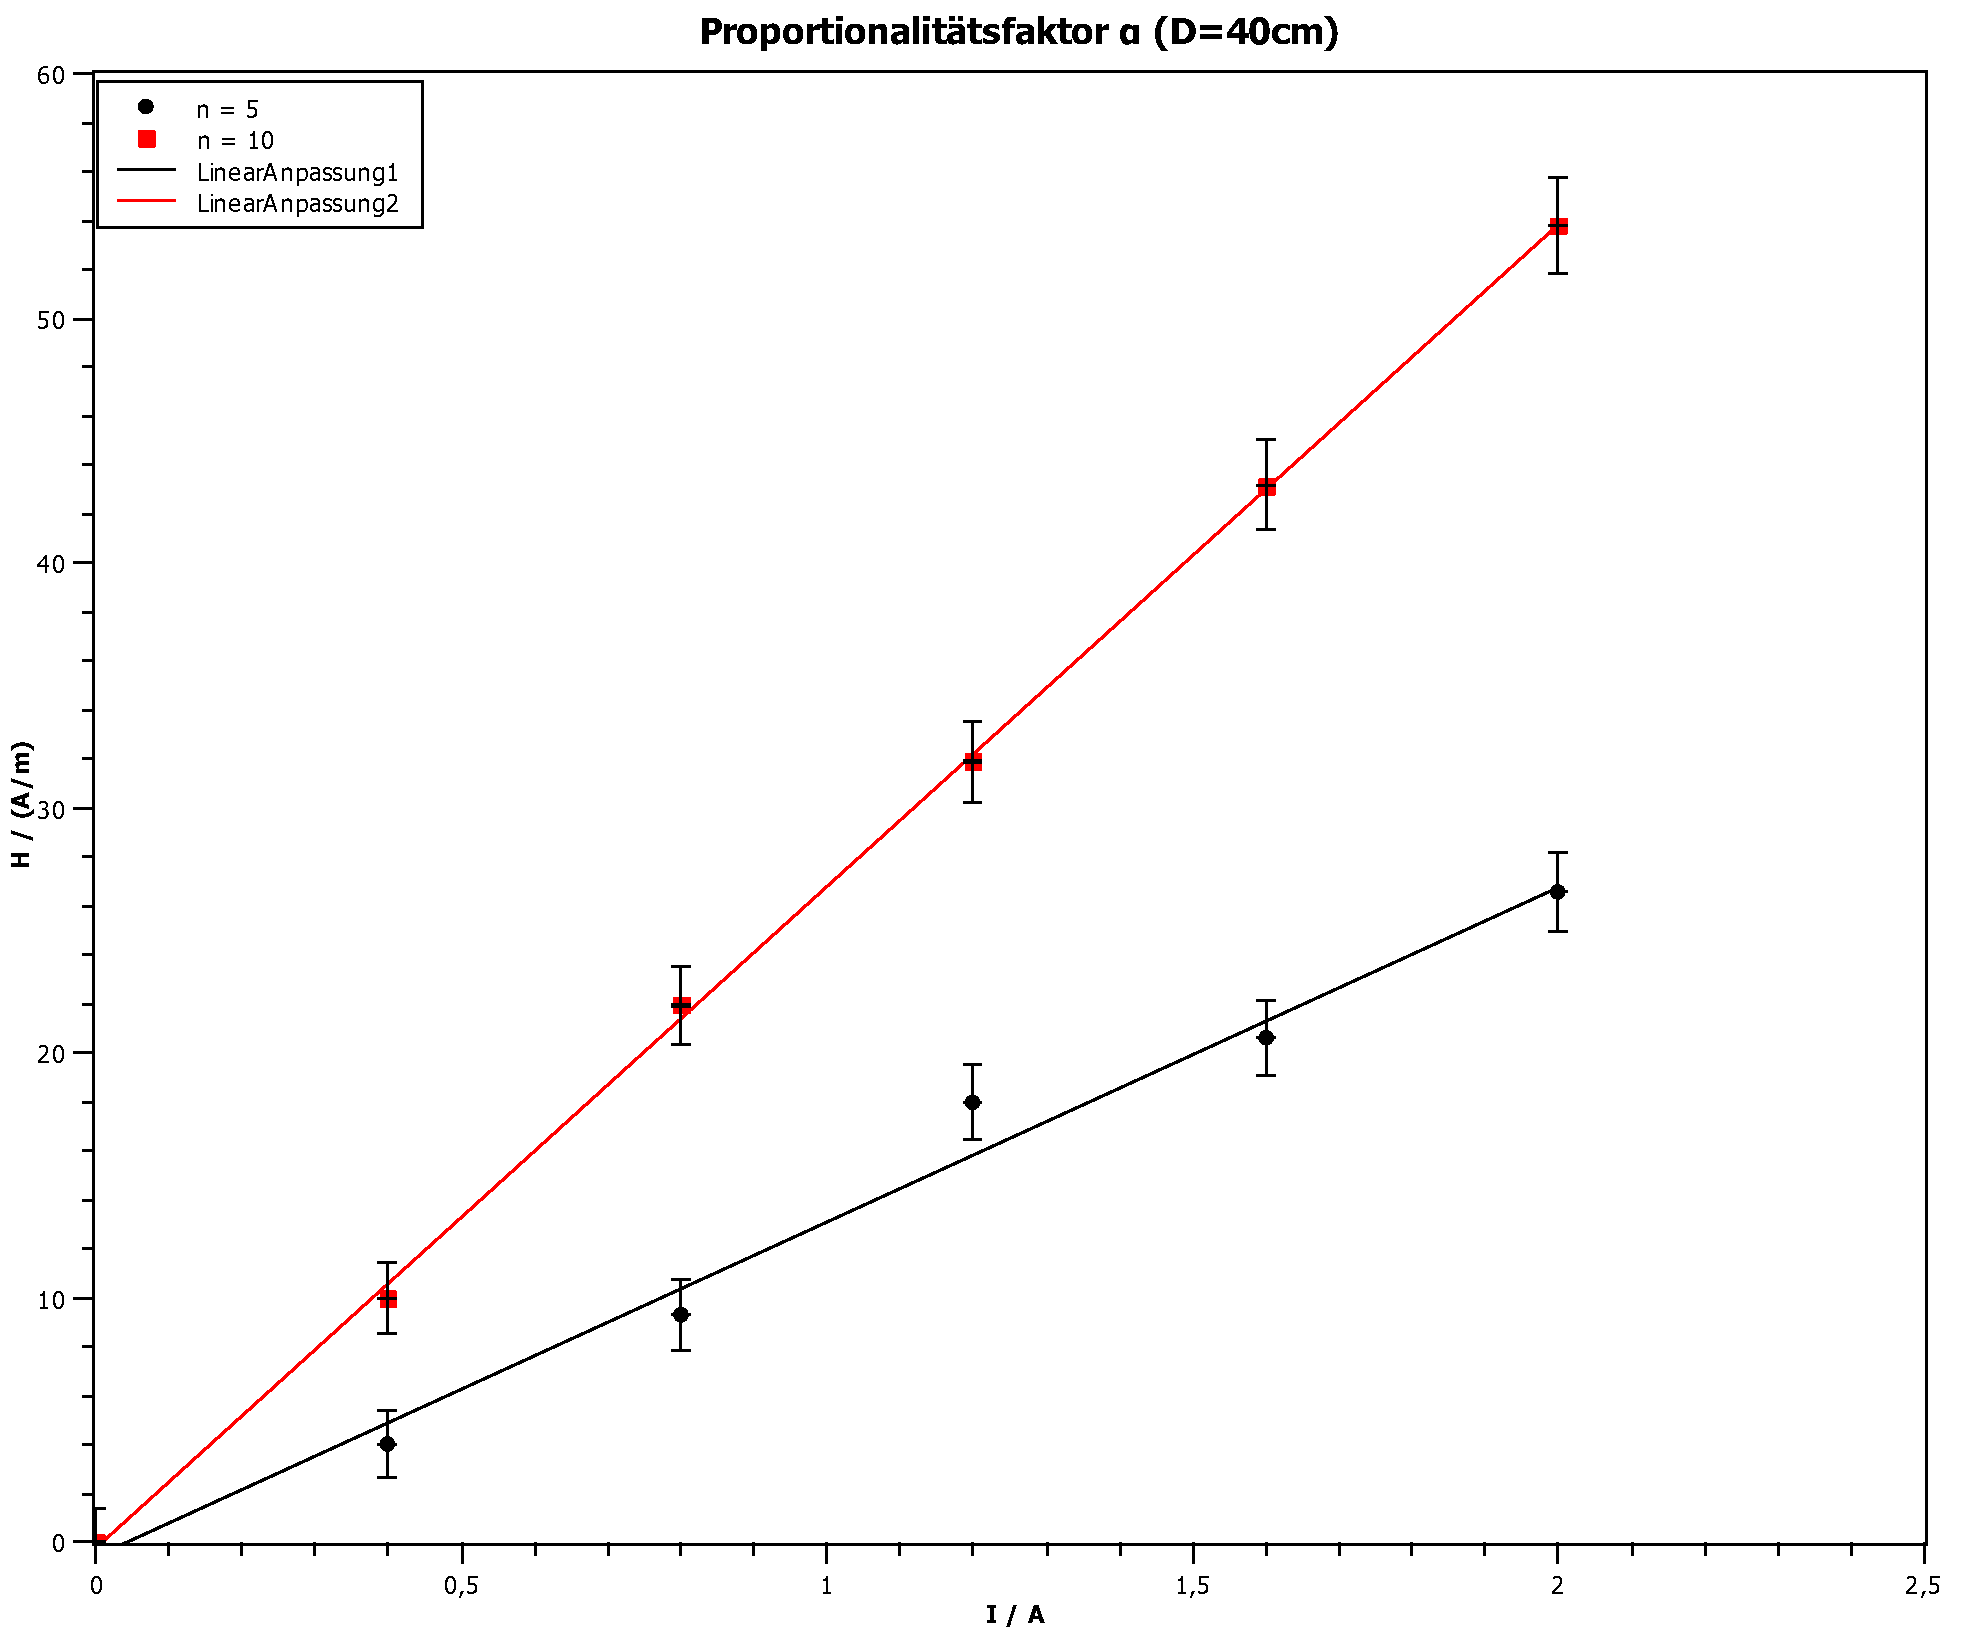
\includegraphics[width=.7\textwidth]{prop40.pdf}
    \caption[Proportionalitätsfaktor für D=40cm]{Proportionalitätsfaktor $\alpha$ für die kurze Spule mit $D=\SI{40}{cm}$.}
    \label{fig:40prop}
\end{figure}

Mit \gl{eq:k} und den gemessenen Ausschlägen für die kurzen Spulen lassen sich ihre magnetische Feldstärken $ H $ ermitteln
und als Funktion des Spulenstroms $ I $ in ein Diagramm (vgl. \bild{fig:20prop} und \bild{fig:40prop}) auftragen. Die
durch eine lineare Anpassunge resultierende Steigung $ m $ liefert mit \gl{eq:4} folgenden Zusammenhang:
\begin{equation}
    m = \frac{H_k}{I} = \alpha \cdot \frac{n}{R}
\end{equation}

und umgestellt nach $ \alpha $:
\begin{equation}
    \alpha = m \cdot \frac{R}{n} = m \cdot \frac{D}{2n}
\end{equation}
$\alpha$ ist hier als Faktor zu verstehen. In \gl{eq:test} wird beispielhaft der Spulenstrom aus \tabelle{tab:mess2} Zeilen Nr. 6
eingesetzt und das resultierende Feld mit dem zuvor ermittelten Kalibrierfaktor multipliziert.
\begin{equation}
    A = \frac{I \cdot N}{R} \cdot k
    = \frac{\SI{1,2}{A} \cdot 10}{\SI{0,1}{m}} \cdot \SI{0,151}{m^{-1}}
    = \SI{18,12}{Skt}
    \label{eq:test}
\end{equation}
Gemessen wurden hier jedoch \SI{10}{Skt}. Die Diskrepanz lässt sich durch die Inhomogenität des Feldes der kurzen Spule
in Kombination mit der Beschaffenheit des Versuchsaufbaus erklären. \gl{eq:4} in \gl{eq:8} eingesetzt zeigt
\begin{equation}
    \varphi = \frac{\phi_1 \cdot s}{d} \cdot \frac{I \cdot n}{R} \quad \Rightarrow \quad \alpha \, \widehat{=} \, \frac{\phi_1 \cdot s}{d}
\end{equation}
Der Wert $\alpha$ korrigiert also um die räumliche Ausdehnung des Stabmagneten, seine eigene Polstärke und den Einfluss
des Direktionsmomentes des Torsionsdrahts.
\par\medskip
Für die vier Messungen an den kurzen Spulen ergeben sich folgende Werte für den Proportionalitätsfaktor $\alpha$:
\vspace{5mm}
\begin{table}[h]
    \centering
    \caption[Proportionalitätsfaktoren]{Steigungen der Ausgleichsgeraden und korrespondierende Werte für den Proportionalitätsfaktor $\alpha$}
    \begin{tabular}{@{}llll@{}}
        \toprule
        \multicolumn{2}{l}{}                       & $(m \pm \Delta m) / m^{-1}$  & $\alpha$ \\ \midrule
        \multirow{2}{*}{$D=\SI{20}{cm}$} & $n=5$   & $27,4 \pm 0,4$               & 0,548    \\
                                         & $n=10$  & $53,1 \pm 0,5$               & 0,531    \\
        \multirow{2}{*}{$D=\SI{40}{cm}$} & $n=5$   & $13,7 \pm 0,8$               & 0,548    \\
                                         & $n=10$  & $27,0 \pm 0,3$               & 0,540    \\ \cmidrule(l){1-4} 
    \end{tabular}
\end{table}

\section{Messunsicherheiten}
Die durch die Messeinrichtung gegebenen Messfehler sind
\begin{align*}
    \Delta L &= \pm \SI{0,001}{m} &\quad& \text{Fehler bei der Längenmessung (Stahllineal).}\\
    \Delta A &= \pm \SI{0,2}{Skt} &\quad& \text{Fehler bei der Auslenkung durch Skalenteilung und Leuchtpunkt.}\\
    \Delta I &= \pm \SI{0,01}{A}  &\quad& \text{Fehler des Spulenstroms durch Ungenauigkeit der Stromquelle.}
\end{align*}

Der größte Fehler für die magnetische Feldstärke $ H $ ergibt sich bei der langen Spule mit der Windungszahl $ n=240 $ gegeben
durch die Messunsicherheiten aus Spulenstrom $I$ und Spulenlänge $L$ zu:
\begin{align}
    \Delta H    &= \left\vert\frac{\delta H}{\delta I}\right\vert \cdot \Delta I + \left\vert\frac{\delta H}{\delta L}\right\vert \cdot \Delta L \nonumber\\
                &= \frac{n}{L} \cdot \Delta I + \frac{n \cdot I}{L^{2}} \cdot \Delta L \nonumber\\
                &= \frac{240}{\SI{0,615}{m}} \cdot \SI{0,01}{A} + \frac{240 \cdot \SI{0,7}{A}}{(\SI{0,615}{m})^2} \cdot \SI{0,001}{m}\nonumber\\
                &= \SI{4,34}{\frac{A}{m}} \nonumber
\end{align}



Der größte Fehler für den Proportionalitätsfaktor $\alpha$ zeigt sich bei der kurzen Spule mit 40 cm Durchmesser und 5 Windungen:
\begin{align}
    \Delta \alpha   &= \left\vert\frac{\delta \alpha}{\delta m}\right\vert \cdot \Delta m \nonumber\\
                    &= \frac{D}{2 \cdot n} \cdot \Delta m \nonumber\\
                    &= \frac{\SI{0,4}{m}}{2 \cdot 5} \cdot \SI{0,8}{m^{-1}} \nonumber\\
                    &= 0,032 \nonumber
\end{align}